\documentclass[12pt]{article}
\usepackage[english]{babel}
\usepackage{natbib}
\usepackage{url}
\usepackage[utf8x]{inputenc}
% https://tex.stackexchange.com/questions/9866/latest-advice-on-the-euro-symbol
\usepackage{lmodern,textcomp}
\usepackage{amsmath}
\usepackage{amsthm}
\usepackage{graphicx}
% https://www.overleaf.com/learn/latex/How_to_Write_a_Thesis_in_LaTeX_(Part_3):_Figures,_Subfigures_and_Tables
\usepackage{caption}
\usepackage{subcaption}
\graphicspath{{images/}}
\usepackage{parskip}
\usepackage{fancyhdr}
\usepackage{vmargin}
\setmarginsrb{3 cm}{2.5 cm}{3 cm}{2.5 cm}{1 cm}{1.5 cm}{1 cm}{1.5 cm}
%https://tex.stackexchange.com/questions/60209/how-to-add-an-extra-level-of-sections-with-headings-below-subsubsection
\usepackage{titlesec}

% Allows usage of [H] in \begin{figure}
\usepackage{float}

% Define custom colors, for example for highlighting filenames
\usepackage{xcolor}
\definecolor{light-gray}{gray}{0.95}

% Links in table of contents
\usepackage{hyperref}
\hypersetup{
	colorlinks=true, %set true if you want colored links
	linktoc=all,     %set to all if you want both sections and subsections linked
	linkcolor=blue,  %choose some color if you want links to stand out
}

% https://tex.stackexchange.com/questions/10684/vertical-space-in-lists
% https://tex.stackexchange.com/questions/2291/how-do-i-change-the-enumerate-list-format-to-use-letters-instead-of-the-defaul
\usepackage[shortlabels]{enumitem}
\setlist{nosep}

% Color boxes
% https://ctan.org/pkg/tcolorbox
\usepackage{tcolorbox}

% For the R for real numbers and other symbols
\usepackage{amssymb}

% https://tex.stackexchange.com/questions/439768/put-reference-above-equal-sign-and-refer-to-it
\newcommand\numeq[1]%
{\stackrel{\scriptscriptstyle(\mkern-1.5mu#1\mkern-1.5mu)}{=}}

% https://tex.stackexchange.com/questions/7350/how-do-i-add-dots-in-toc
\usepackage{tocloft}
\renewcommand{\cftsecleader}{\cftdotfill{\cftdotsep}}

% https://tex.stackexchange.com/questions/28836/typesetting-the-define-equals-symbol
\usepackage{mathtools}
\newcommand{\defeq}{\vcentcolon=}
\newcommand{\eqdef}{=\vcentcolon}

% https://tex.stackexchange.com/questions/159257/increase-latex-table-row-height
{\renewcommand{\arraystretch}{2}

% https://www.overleaf.com/learn/latex/Environments
\theoremstyle{definition}
\newtheorem{example}{Example}[section]
\theoremstyle{definition}
\newtheorem{definition}{Definition}[section]
\theoremstyle{theorem}
\newtheorem{theorem}{Theorem}
\newtheorem{prop}{Proposition}

% Commonly used symbols
\newcommand{\R}{\mathbb{R}} % Real numbers
\renewcommand{\P}{\mathrm{P}} % Probability
\newcommand{\F}{\mathcal{F}} % A sigma-algebra
\renewcommand{\O}{\Omega} % The sample space
\newcommand{\PS}{(\O, \F, \P)} % The probability space


%%%%%%%%%%%%%%%%%%%%%%%%%%%%%%%%%%%%%%%%%%%%%%%%%%%%%%%%%%%%%%%%%%%%%%%


\title{Handbook of Statistics}
\author{David Silva Sanmartín}
\date{\today}

\makeatletter
\let\thetitle\@title
\let\theauthor\@author
\let\thedate\@date
\makeatother

\pagestyle{fancy}
\fancyhf{}
\rhead{\theauthor}
\lhead{\thetitle}
\cfoot{\thepage}

\begin{document}

	% Make all the references appear always
	\nocite{*}

	%%%%%%%%%%%%%%%%%%%%%%%%%%%%%%%%%%%%%%%%%%%%%%%%%%%%%%%%%%%%%%%%%%%%%%%%%%%%%%%%%%%%%%%%%
	
	\begin{titlepage}
		\centering
		\vspace*{0.5 cm}
		
\includegraphics[scale = 0.2]{uned.jpg}\\[1.0 cm] % University Logo
		\textsc{\LARGE Mathematics}\\[2.0 cm] % University Name
		%\textsc{\Large Modelización}\\[0.5 cm] % Course Code
		%\textsc{\large Herramientas Informáticas Para Matemáticas}\\[0.5 cm] % Course Name
		\rule{\linewidth}{0.2 mm} \\[0.4 cm]
		{ \huge \bfseries \thetitle}\\
		\rule{\linewidth}{0.2 mm} \\[1.5 cm]
		
		\begin{minipage}{0.4\textwidth}
			\begin{flushleft} \large
				\emph{Author:}\\
				\theauthor
			\end{flushleft}
		\end{minipage}~
		\begin{minipage}{0.4\textwidth}
			\begin{flushright} \large
			\end{flushright}
		\end{minipage}\\[2 cm]
		
		{\large \thedate}\\[2 cm]
		
		\vfill
		
	\end{titlepage}
	
	%%%%%%%%%%%%%%%%%%%%%%%%%%%%%%%%%%%%%%%%%%%%%%%%%%%%%%%%%%%%%%%%%%%%%%%%%%%%%%%%%%%%%%%%%
	
	\tableofcontents
	\pagebreak
	
	%%%%%%%%%%%%%%%%%%%%%%%%%%%%%%%%%%%%%%%%%%%%%%%%%%%%%%%%%%%%%%%%%%%%%%%%%%%%%%%%%%%%%%%%%
	
	\part{Theory}
	\section{Probability spaces}
	% TODO: sigma-algebras...

\subsection{Definition and basic properties}

\begin{definition}
	\textbf{Random Experiment:} an experiment whose outcomes are determined only by chance factors.
\end{definition}

\begin{definition}
	The description of a random experiment starts by identifying the set of all possible  outcomes of the experiment, which we call \textbf{sample space}, and we designate by $\O$.
	\begin{itemize}
		\item When $\O$ is finite or countable (\textit{numerable}), we say that the probability model is \textbf{discrete}.
		\item When $\O$ is uncountable, we say that the probability model is \textbf{continuous}.
	\end{itemize}
\end{definition}

\begin{definition}
	Let $\O$ be a set and $\F$ a $\sigma$-algebra on $\O$. We say that $(\O, \F)$ is a \textbf{measurable space}. Any subset belonging to $\F$ is called an \textbf{event}.
	\begin{itemize}
		\item When $\O$ is finite or countable, we will usually consider $\F = \mathcal{P}(\O)$.
		\item When $\O$ is uncountable, with $\O \subseteq \R^k$, we will usually consider $\F = \mathbb{B}_{\O}^k$.
	\end{itemize}
\end{definition}

\begin{definition}
	Given a measurable space $(\O, \F)$, a \textbf{probability}, or \textbf{probability measure}, is a function $\P: \F \rightarrow \R$ such that:
	\begin{enumerate}[i)]
		\item $\P(A) \geq 0$ for every $A \in \F$.
		\item For every countable collection of events $\{A_n\} \subset \F$, which are pairwise disjoint, we have that:
		\[
			\P \left(\cup_n A_n\right) = \sum_n \P(A_n)
		\]
		\item $\P(\O) = 1$
	\end{enumerate}
	If $\P$ is a probability in $(\O, \F)$, we call the triad $(\O, \F, \P)$ a \textbf{probability space}. For every event $A \in \F$, we call $\P(A)$ the \textbf{probability of $A$}.
\end{definition}

\begin{prop}
	Let $(\O, \F, \P)$ be a probability space, and $A, B \in \F$. Then:
	\[
		\P(A - B) = \P(A) - \P(A \cap B)
	\]
	If $B \subseteq A$, then
	\[
		\P(A - B) = \P(A) - \P(B)
	\]
	and, thus, $\P(B) \leq \P(A)$. In particular, it is $\P(A) \leq 1$ for every $A \in \F$, and:
	\[
		\P(A^c) = 1 - \P(A)
	\]
	And from this last equality we deduce that $\P(\emptyset) = 0$.
\end{prop}

\begin{prop}
	Let $(\O, \F, \P)$ be a probability space, and $A_1, \ldots, A_n \in \F$. Then,
	\[
		\P(A_1 \cup A_2) = \P(A_1) + \P(A_2) - \P(A_1 \cap A_2)
	\]
	and, more generally, the \textbf{inclusion-exclusion formula} holds:
	\[
		\begin{gathered}
		\P(\cup_{i = 1}^n A_i) = \sum_{i = 1}^n\P(A_i) - \sum_{1 \leq i \leq j \leq n}\P(A_i \cap A_j) + \sum_{1 \leq i \leq j \leq k \leq n} \P(A_i \cap A_j \cap A_k) \\ + \cdots + (-1)^{n - 1} \P(A_1 \cap A_2 \cap \cdots A_n)
		\end{gathered}
	\]
\end{prop}

\subsection{Conditional probability}

In a probability space $(\O, \F, \P)$, the fact of knowing that the outcome of the random experiment verifies a particular event $B$, affects the probability of all events.
% TODO: find better explanation ...

\begin{definition}
	Let $B \in \F$ be an event such that $\P(B) > 0$. For each $A \in \F$, we define the \textbf{conditional probability of $A$ given $B$} as:
	\[
		\P(A \mid B) = \frac{\P(A \cap B)}{\P(B)}
	\]
\end{definition}

The knowledge that the event $B$ has been verified transforms the original probability space into a new one, $(\O, \F, \P(\cdot \mid B))$. Because we also know that the event $B^c$ has not happened, we can consider a more relevant space, $(B, \F_B, \P_B)$, in which:
\[
	\F_B = \{ A \cap B \mid A \in \F \}
\]
is the new $\sigma$-algebra of events. We assign each of the new events, $C \in \F_B$, the probability:
\[
	\P_B(C) = \frac{\P(C)}{\P(B)} = \frac{\P(A \cap B)}{\P(B)}, \text{ if } C = A \cap B \text{ for some } A \in \F
\]

\begin{prop}
	Let $(\O, \F, \P)$ be a probability space. If $B \in \F$ is an event such that $\P(B) > 0$, then both $(\O, \F, \P(\cdot \mid B))$ and $(B, \F_B, \P_B)$ are probability spaces.
\end{prop}

\begin{prop}[Product rule or Chain rule]
	Let $\PS$ be a probability space, and $A_1, \ldots, A_n \in \F$ events such that $\P(\cap_{i = 1}^{n - 1} A_i) > 0$. Then,
	\[
		\P(\cap_{i = 1}^{n} A_i) = \P(A_1) \P(A_2 \mid A_1) \P(A_3 \mid A_2 \cap A_1) \cdots \P(A_n \mid \cap_{i = 1}^{n - 1} A_i)
	\]
\end{prop}
\begin{proof}
	By iteratively applying the definition of conditional probability, $\P(A \cap B) = \P(B) \P(A \mid B)$, we have that:
	\begin{align*}
		\P(\cap_{i = 1}^{n} A_i) &= \P(\cap_{i = 1}^{n - 1} A_i)\P(A_n \mid \cap_{i = 1}^{n - 1}) = \\
		 &= \P(\cap_{i = 1} ^{n - 2} A_i) \P(A_{n - 1} \mid \cap_{i = 1} ^{n - 2} A_i) \P(A_n \mid \cap_{i = 1}^{n - 1}) = \\
		 &= \cdots
	\end{align*}
\end{proof}

\begin{prop}[Law or formula of total probability]
	If ${B_n} \subset \F$ is a finite or countably infinite partition of the sample space (in other words, a set of pairwise disjoint events whose union is $\O$) and $\P(B_n) > 0$ for each $n$, then for any event $A \in \F$:
	\[
		\P(A) = \sum_n \P(B_n) \P(A \cap B_n)
	\]
\end{prop}
\begin{proof}
	\begin{align*}
		\P(A) &= \P(A \cap \O) = \P(A \cap (\cup_n B_n)) = \P(\cup_n (A \cap B_n)) = \sum_n \P(A \cap B_n) = \\ &= \sum_n \P(B_n) \P(A \cap B_n)
	\end{align*}
\end{proof}

\begin{prop}[Bayes' formula]
	If $A$ and $B$ are events in the probability space $\PS$ such that $\P(B) > 0$, then:
	\[
		\P(A \mid B) = \frac{\P(A) \, \P(B \mid A)}{\P(B)}
	\]
\end{prop}

\begin{proof}
	\[
		\P(A \mid B) = \frac{\P(A \cap B)}{\P(B)} = \frac{\P(A) \, \P(B \mid A)}{\P(B)}
	\]
\end{proof}

\subsection{Independence}

\begin{definition}
	Let $\PS$ be a probability space. $\{ A_i \}_{i \in I }$ are \textbf{independent events} if:
	\[
		\P (\cap_{i \in F} A_i) = \prod_{i \in F} \P(A_i)
	\]
	for every finite subset $F \subset I$.
\end{definition}

\begin{definition}
	Let $\PS$ be a probability space and $\{ \mathcal{C}_i \}_{i \in I}$ families of events, where $\mathcal{C}_i \subset \F$ for each $i \in I$. $\{ \mathcal{C}_i \}_{i \in I}$ are said to be \textbf{independent} if the events $\{ A_i \}_{i \in I }$ are independent for every election of $A_i \in \mathcal{C}_i$ for every $i \in I$.
\end{definition}

\begin{example}
	Exercise 3.7 ...
\end{example}
	\newpage
	
	\section{Random variables}
	\subsection{Random variables and expectations}

\begin{definition}
	\textbf{Random Experiment:} an experiment whose outcomes are determined only by chance factors.
\end{definition}

\begin{definition}
	\textbf{Sample Space:} the set of all possible outcomes of a random experiment.
\end{definition}

\begin{definition}
	\textbf{Event:} the collection of none, one, or more than one outcomes from a sample space.
\end{definition}

\begin{definition}
	\textbf{Random Variable}: a variable whose numerical values are determined by chance factors. It is a function from the sample space to a set of real numbers.
\end{definition}
Given a sample space $\Omega = \{ \omega_1, \ldots, \omega_n \}$ with probability function $P$ and a random variable $X$ with range $\mathbb{X} = \{ x_1, \ldots x_m \}$, we can define a probability function $P_X$ on $\mathbb{X}$ in the following way: We will observe $X = x_i$ if and only if the outcome of the random experiment is an $\omega_i \in \Omega$ such that $X(\omega_j) = x_i$. Thus,
\[
	P_X(X = x_i) = P(\{ \omega_j \in \Omega \mid X(\omega_j) = x_i \})
\]
The function $P_X$ is an \textit{induced} probability function on $\mathbb{X}$, defined in terms of the orginal function $P$. We will write $P(X = x_i)$ rather than $P_X(X = x_i)$.
\begin{definition}
	\textbf{Discrete Random Variable:} if the set of all possible values of a random variable $X$ is countable, then $X$ is called a \textit{discrete random variable}.
\end{definition}

\begin{definition}
	\textbf{Probability Mass Function (pmf):} let $R$ be the set of all possible values of a discrete random variable $X$, and $f(k) = P(X = k)$ for each $k$ in $R$. Then $f(k)$ is called the \textit{probability mass function} of $X$.
\end{definition}

\begin{definition}
	\textbf{Continuous Random Variable:} if the set of all possible values of $X$ an interval or union of two or more nonoverlapping intervals in $\mathbb{R}$, then $X$ is called a \textit{continuous random variable}.
\end{definition}

\begin{definition}
	\textbf{Probability Density Function (pdf):} any real valued function $f(x)$ that satisfies the following requirements is called a \textit{probability density function}:
	\[
		f(x) \geq 0 \text{ for all } x, \text{ and } \int_{-\infty}^{\infty}f(x)\,dx = 1
	\]
\end{definition}

\begin{definition}
	\textbf{Cumulative Distribution function (cdf):} the \textit{cumulative distribution function} of a random variable $X$ is defined by
	\[
		F(x) = P(X \leq x)
	\]
	For a continuous random variable $X$ with the probability density function $f(x)$,
	\[
	F(x) = P(X \leq x) = \int_{-\infty}^x f(t)\,dt, \ \forall x
	\]
	For a discrete random variable $X$, the \textit{cdf} is defined by
	\[
	F(k) = P(X \leq k) = \sum_{i = -\infty}^k P(X = i)
	\]
\end{definition}
The \textit{pdf} (or \textit{pmf}) contains the same information as the \textit{cdf}.

If the distribution of a random variable $X$ depends on a parameter $\theta$, the the \textit{pdf} or \textit{pmf} of $X$ is usually expressed as $f(x \mid \theta)$, and the \textit{cdf} is written as $F(x \mid \theta)$
\begin{theorem}
	A function $F(x)$ is a cdf if and only if the following three conditions hold:
	\begin{enumerate}[\bfseries a)]
		\item $\lim_{x \rightarrow -\infty}F(x) = 0$ and $\lim_{x \rightarrow \infty}F(x) = 1$.
		\item $F(x)$ is a nondecreasing function of x.
		\item $F(x)$ is right-continuous; that is, for every number $x_0$, $\lim_{x \rightarrow x_0^{+}} F(x) = F(x_0)$
	\end{enumerate}
\end{theorem}

\begin{definition}
	\textbf{Expectation:} if $X$ is a continuous random variable with the \textit{pdf} $f(x)$, then the expectation of $g(X)$, where $g$ is a real valued function, is defined by
	\[
		E(g(X)) = \int_{-\infty}^{\infty}g(x)f(x)\,dx
	\]
	If $X$ is a discrete random variable, then
	\[
		E(g(X)) = \sum_k g(x) P(X = k)
	\]
	where the sum is over all possible values of $X$. Thus, $E(g(X))$ is the weighted average of the possible values of $g(X)$, each weighted by its probability.
\end{definition}

\begin{theorem}
	Let $X$ be a random variable and let a, b and c be constants. Then for any functions $g_1(x)$ and $g_2(x)$ whose expectations exist,
	\begin{enumerate}[\bfseries a)]
		\item $E(ag_1(X) + bg_2(X) + c) = aEg_1(X) + bEg_2(X) + c$.
		\item If $g_1(x) \geq 0 \ \forall x$, then $Eg_1(X) \geq 0$.
		\item If $g_1(x) \geq g_2(x) \ \forall x$, then $Eg_1(X) \geq Eg_2(X)$.
		\item If $a \leq g_1(x) \leq b \ \forall x$, then $a \leq Eg_1(X) \leq b$. 
	\end{enumerate}
\end{theorem}

\subsection{Measures of Central Tendency}

\begin{definition}
	\textbf{Mean:} the \textit{mean} of a random variable $X$ is usually denoted by $\mu$. For a discrete random variable $X$, it is defined by
	\[
		\mu = E(X) = \sum_{k}P(X = k)
	\]
	where the sum is over all possible values of $X$. For a continuous random variable $X$ with probability density function $f(x)$, the \textit{mean} is defined by
	\[
		\mu = E(X) = \int_{-\infty}^{\infty} xf(x) \, dx
	\]
\end{definition}

\begin{definition}
	\textbf{Median:} the \textit{median} of a random variable $X$ is the value such that 50\% of the possible values of $X$ are less than or equal to that value. For a discrete distribution, median is not well defined, and it need not be unique.
\end{definition}

\begin{definition}
	\textbf{Mode:} the most probable value of the random variable.
\end{definition}

\subsection{Moments}

\begin{definition}
	\textbf{Moments about the origin (Raw Moments)}: for each integer $n$, the $n$th \textit{moment} of $X$ (or $F(X)$), $\mu_n'$, is
	\[
		\mu_n' = EX^n
	\]
	For a continuous random variable this is:
	\[
		\mu_n' = EX^n = \int_{-\infty}^{\infty} x^n f(x) \, dx
	\]
	We can see that the mean is $\mu = \mu_1' = EX$.
\end{definition}

\begin{definition}
	\textbf{Moments about the mean (Central Moments):} for each integer $n$, the $n$th \textit{central moment} of $X$ (or $F(X)$), $\mu_n$, is
	\[
		\mu_n = E(X - \mu)^n
	\]
\end{definition}

\begin{definition}
	\textbf{Variance:} the \textit{variance} of a random variable $X$ is its second central moment:
	\[
		\sigma^2 = VarX = E(X - EX)^2
	\]
	An alternative formula for the variance is given by
	\[
		VarX = EX^2 - (EX)^2
	\]
\end{definition}

\begin{definition}
	\textbf{Standard deviation:} the \textit{standard deviation} of a random variable $X$ is the square root of $Var X$:
	\[
		\sigma = \sqrt{VarX}
	\]
\end{definition}

The variance gives a measure of the degree of spread of a distribution around its mean. Larger values mean $X$ is more variable. At the extreme, if $VarX = E(X - EX)^2 = 0$, then $X$ is equal to $EX$ with probability 1, and there is no variation in $X$.

The standard deviation has the same qualitative interpretation: small values mean $X$ is very likely to be close to $EX$, and large values mean $X$ is very variable. The standard deviation is easier to interpret in that the measurement unit on the standard deviation is the same as that for the original variable $X$.

\begin{theorem}
	If $X$ is a random variable with finite variance, then for any constants $a$ and $b$:
	\[
		Var(aX + b) = a^2 VarX
	\]
\end{theorem}

\begin{definition}
	\textbf{}
\end{definition}
\begin{definition}
	\textbf{}
\end{definition}
	\newpage
	
	\part{Discrete distributions}
	\section{Discrete uniform distribution}
	%\begin{figure}[H]
%	\centering
%	\includegraphics[width=\textwidth]{pr0201.png}
%\end{figure}
\subsection{Description}
Used to model experimental outcomes which are "equally likely".

\subsubsection{Probability mass function}
$$P(X=k)=\frac{1}{N},\quad k=1,\ldots,N$$

\subsubsection{Cumulative distribution function}
$$P(X \leq k)=\frac{k}{N},\quad k=1,\ldots,N$$

\subsubsection{Plot}

\subsection{Moments}
\begin{center}
	\begin{tabular}{l l}
		Mean & $\frac{N+1}{2}$ \\
		Variance & $\frac{(N-1)(N+1)}{2}$\\
	\end{tabular}
\end{center}

	\newpage
	
	\section{Binomial distribution}
	\section{Description}

A binomial experiment involves $n$ independent and identical trial such that each trial can result into one of the two possible outcomes: success of failure. If $p$ is the probability of observing success in each trial, then the number of successes $X$ that can be observed out of these $n$ trials is referred to as the \textbf{binomial random variable with $n$ trials and success probability $p$}, or $B(n, p)$.

Binomial distribution is often used to estimate or determine the proportion of individuals with a particular attribute in a large population. Suppose that a random sample of $n$ units is drawn by sampling with replacement from a finite population or by sampling without replacement from a large population. The number of units that contain the attribute of interest in the sample follows a normal distribution.

If the sample was drawn without replacement from a small finite population, the hypergeometric distribution should be used instead of the binomial.

\subsection{Probability mass function}
The probability of observing $k$ successes out of $n$ trials is given by the following probability mass function
\[
	P(X = k \mid n, p) = \binom{n}{k}p^{k}(1 - p)^{n - k}, \quad k = 0, 1, \ldots, n
\]

Binomial's pmf is right-skewed when $p < 0.5$, left-skewed when $p > 0.5$ and symmetric when $p = 0.5$.

% For the future: on image and floats positioning
% https://tex.stackexchange.com/questions/278727/split-subfigures-over-multiple-pages/278748
% https://tex.stackexchange.com/questions/16207/image-from-includegraphics-showing-up-in-wrong-location/16211
\begin{figure}[H]
	\centering
	\begin{subfigure}[b]{0.45\textwidth}
		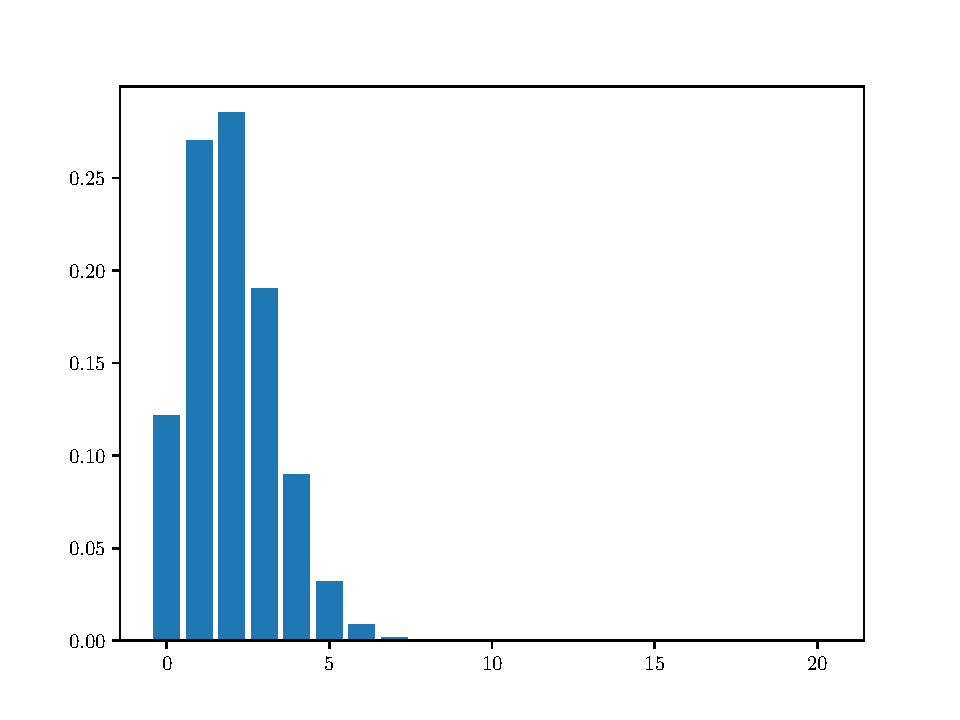
\includegraphics[width=\textwidth]{discrete/binomial/pmf_20_01.pdf}
		\caption{$B(20, 0.1)$}
	\end{subfigure}
	\begin{subfigure}[b]{0.45\textwidth}
		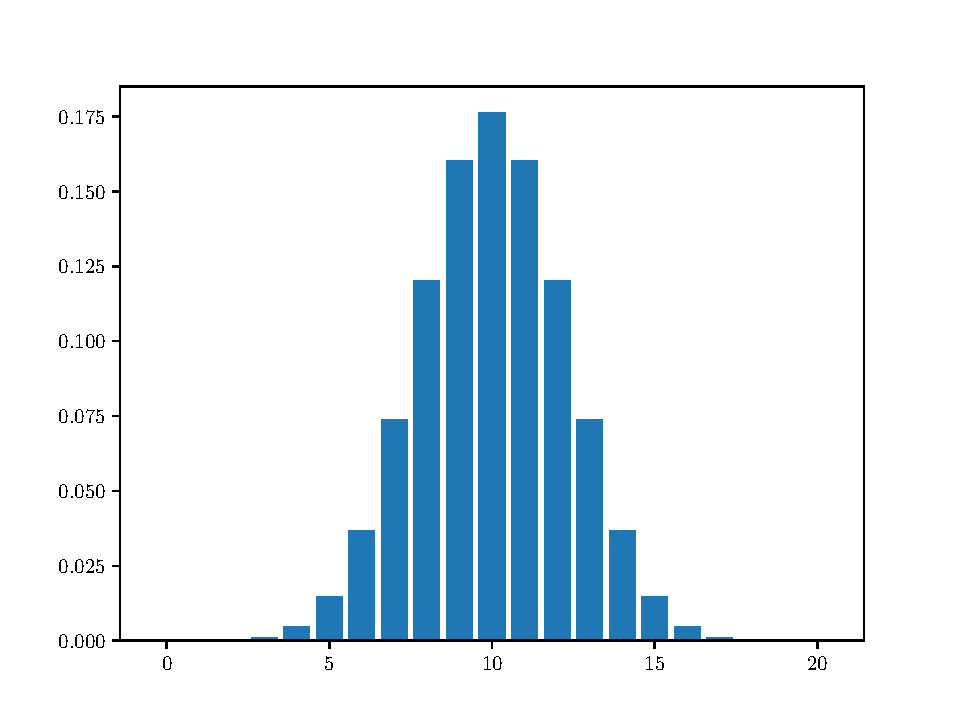
\includegraphics[width=\textwidth]{discrete/binomial/pmf_20_05.pdf}
		\caption{$B(20, 0.5)$}
	\end{subfigure}
	\begin{subfigure}[b]{0.45\textwidth}
		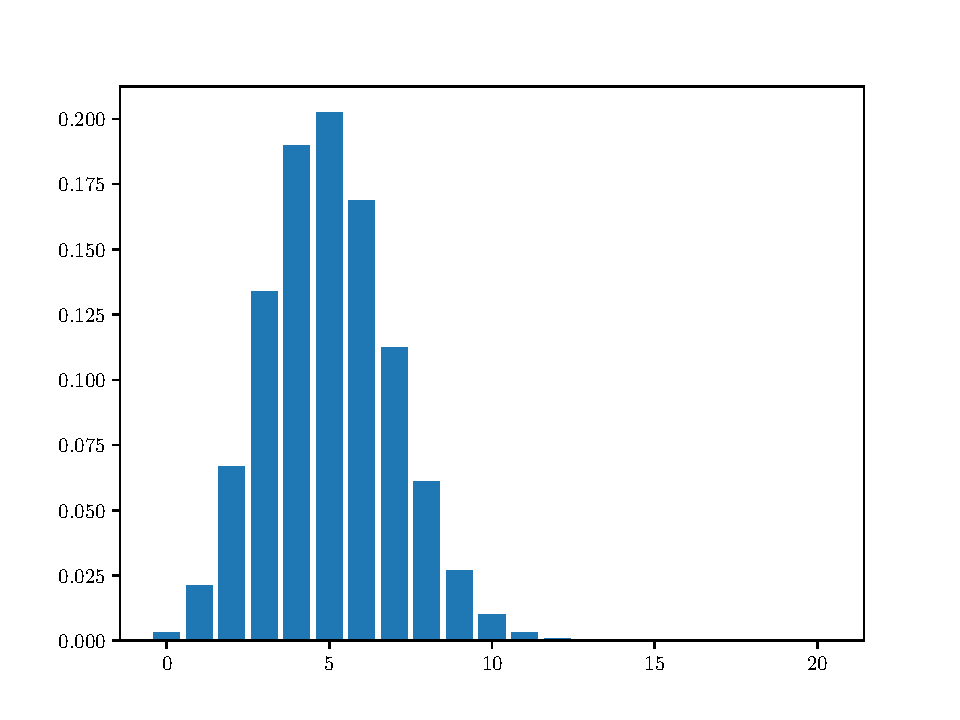
\includegraphics[width=\textwidth]{discrete/binomial/pmf_20_025.pdf}
		\caption{$B(20, 0.25)$}
	\end{subfigure}
	\begin{subfigure}[b]{0.45\textwidth}
		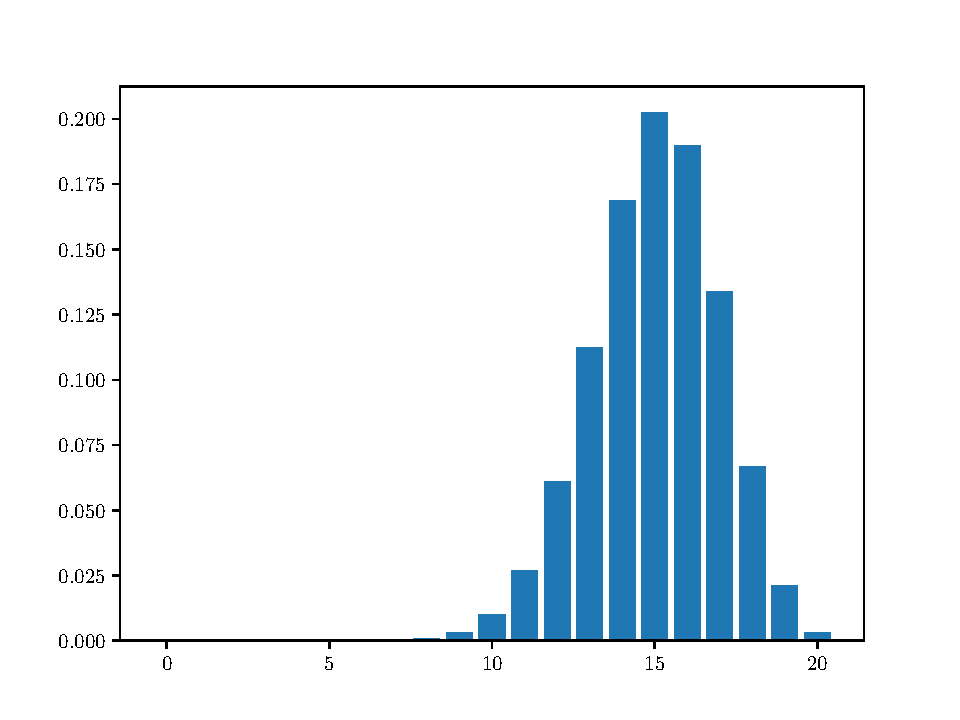
\includegraphics[width=\textwidth]{discrete/binomial/pmf_20_075.pdf}
		\caption{$B(20, 0.75)$}
	\end{subfigure}
	\begin{subfigure}[b]{0.45\textwidth}
		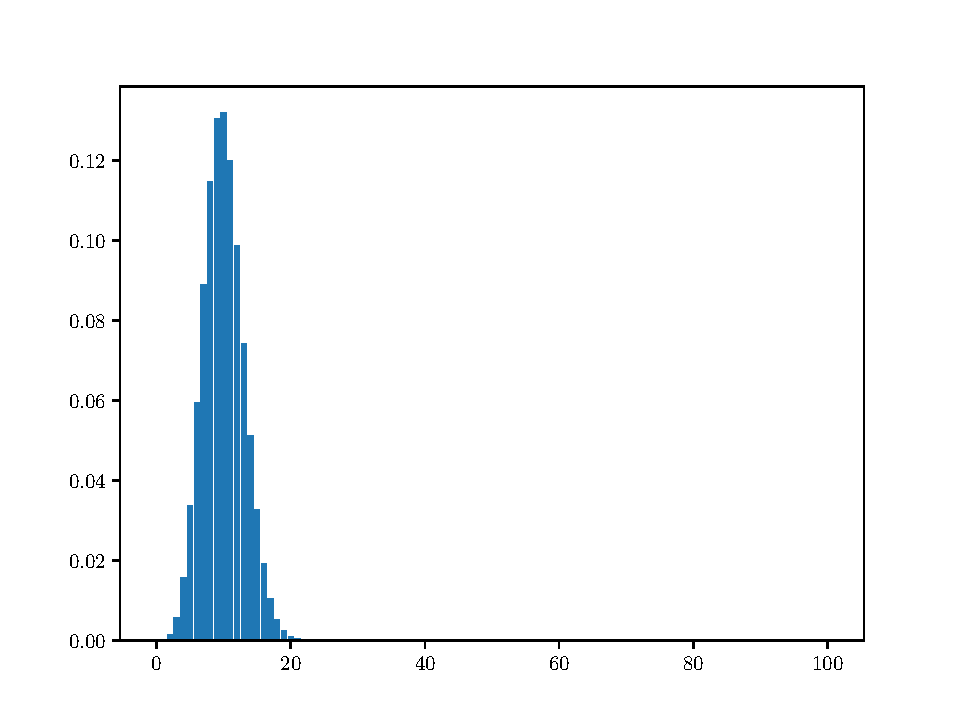
\includegraphics[width=\textwidth]{discrete/binomial/pmf_100_01.pdf}
		\caption{$B(100, 0.1)$}
	\end{subfigure}
	\begin{subfigure}[b]{0.45\textwidth}
		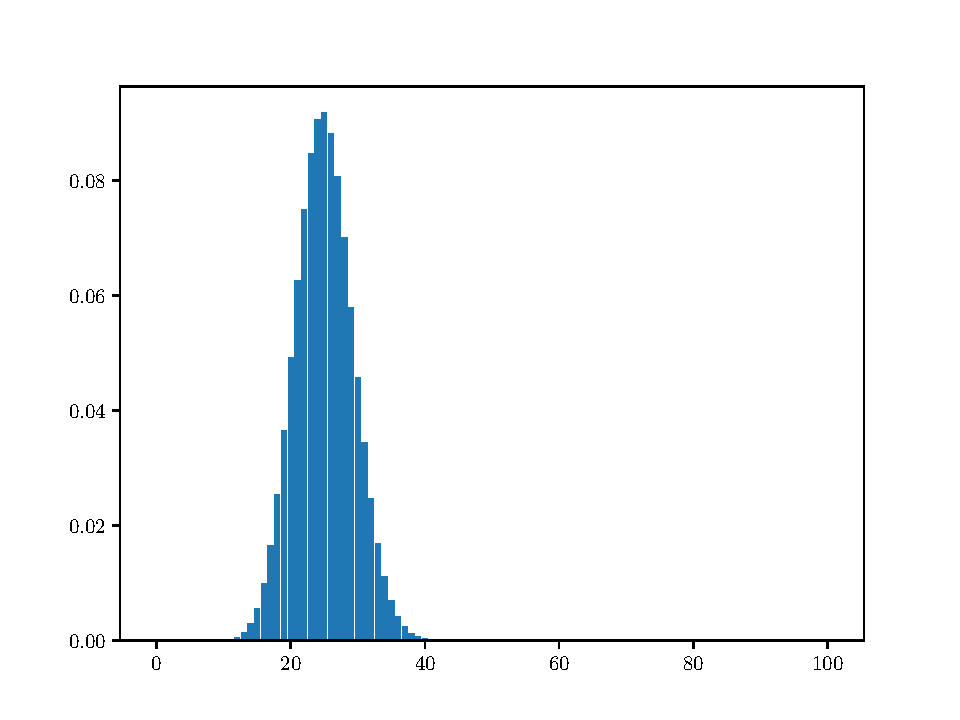
\includegraphics[width=\textwidth]{discrete/binomial/pmf_100_025.pdf}
		\caption{$B(100, 0.25)$}
	\end{subfigure}
	\caption{Binomial distribution}
\end{figure}

\begin{figure}[H]
	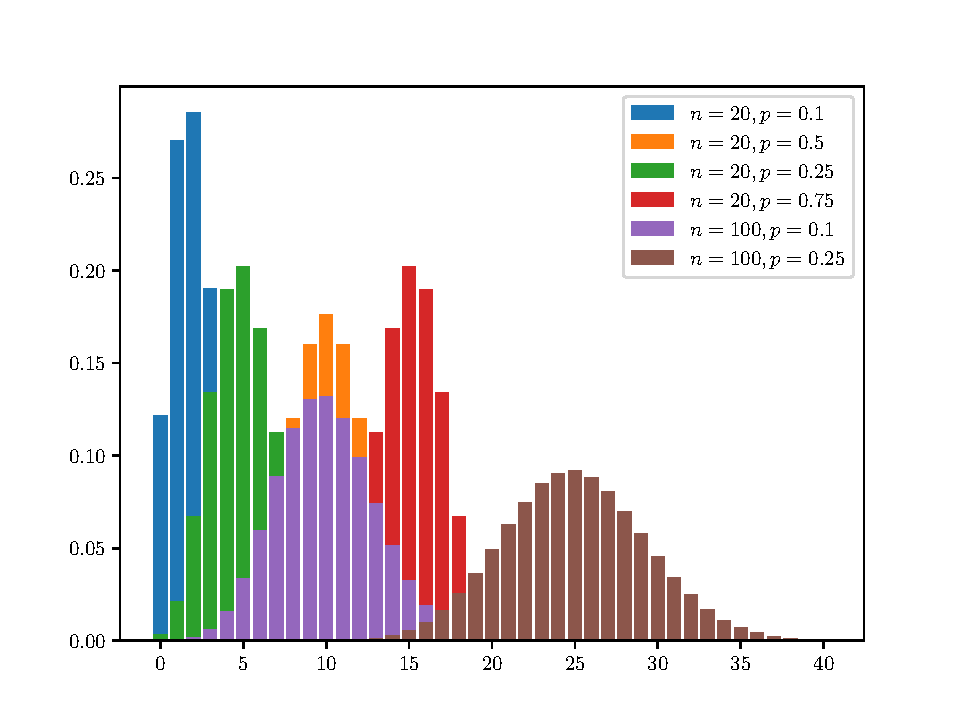
\includegraphics[width=\textwidth]{discrete/binomial/pmf_all.pdf}
	\caption{$P(X = k \mid n, p) = \binom{n}{k}p^{k}(1 - p)^{n - k}, \quad k = 0, 1, \ldots, n$}
\end{figure}

\subsection{Cumulative distribution function}
\[
	P(X \leq k \mid n, p) = \sum_{i = 0}^{k} \binom{n}{i}p^{i}(1 - p)^{n - i}, \quad k = 0, 1, \ldots, n
\]

\begin{figure}[H]
	\centering
	\begin{subfigure}[b]{0.45\textwidth}
		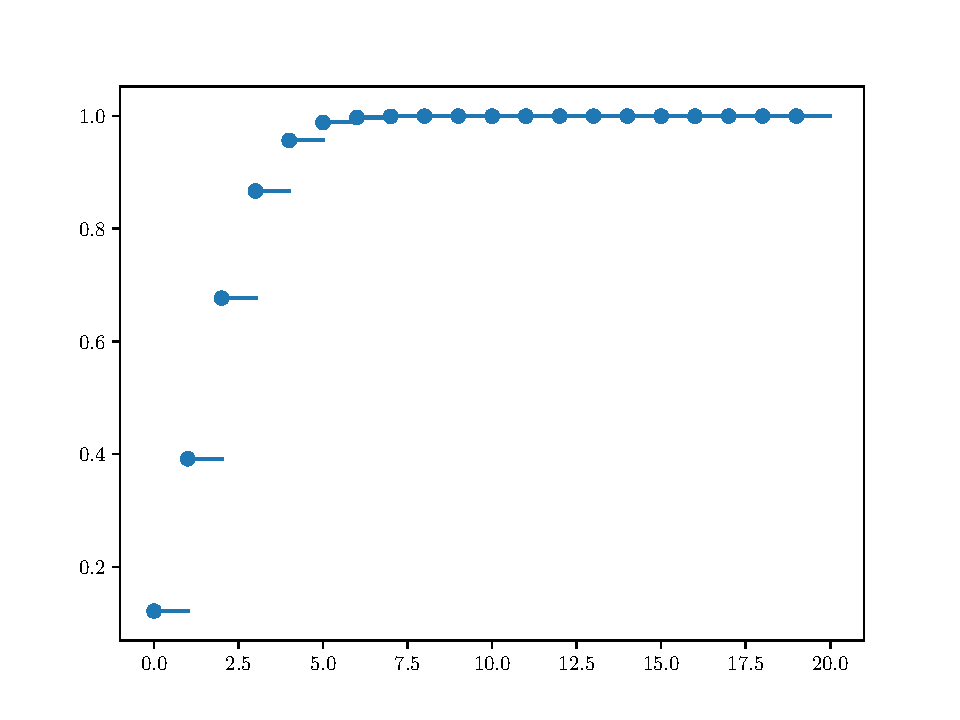
\includegraphics[width=\textwidth]{discrete/binomial/cdf_20_01.pdf}
		\caption{$B(20, 0.1)$}
	\end{subfigure}
	\begin{subfigure}[b]{0.45\textwidth}
		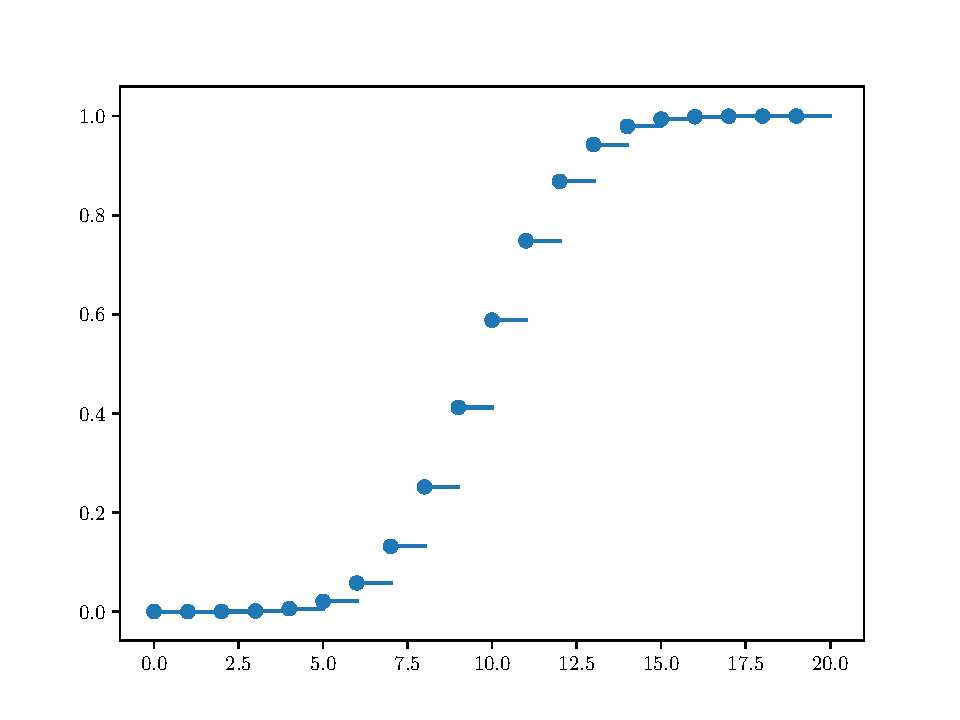
\includegraphics[width=\textwidth]{discrete/binomial/cdf_20_05.pdf}
		\caption{$B(20, 0.5)$}
	\end{subfigure}
	\begin{subfigure}[b]{0.45\textwidth}
		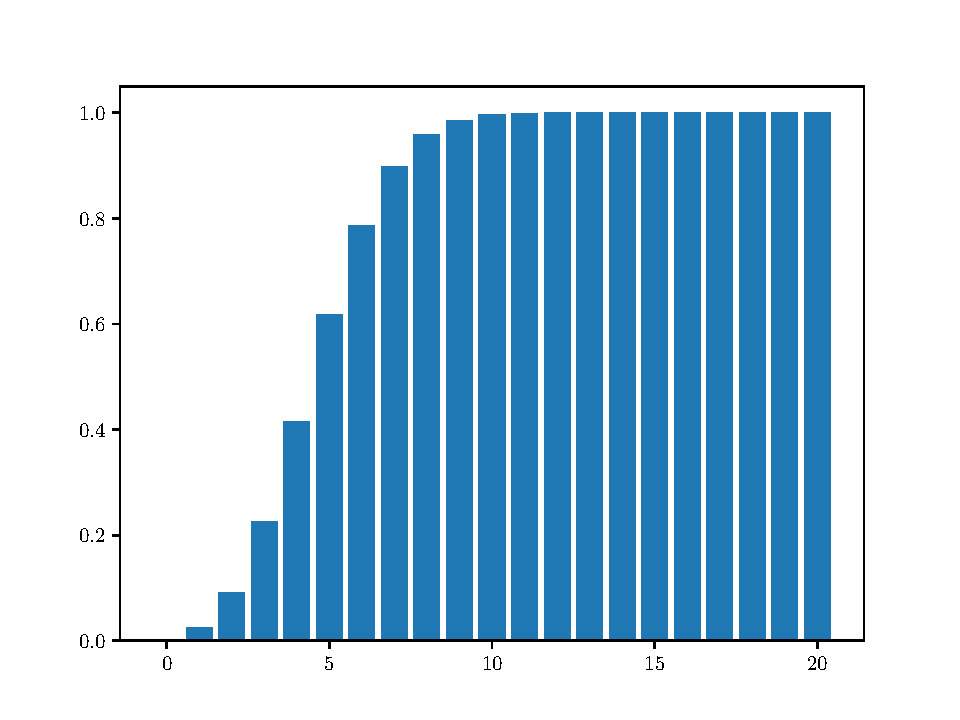
\includegraphics[width=\textwidth]{discrete/binomial/cdf_20_025.pdf}
		\caption{$B(20, 0.25)$}
	\end{subfigure}
	\begin{subfigure}[b]{0.45\textwidth}
		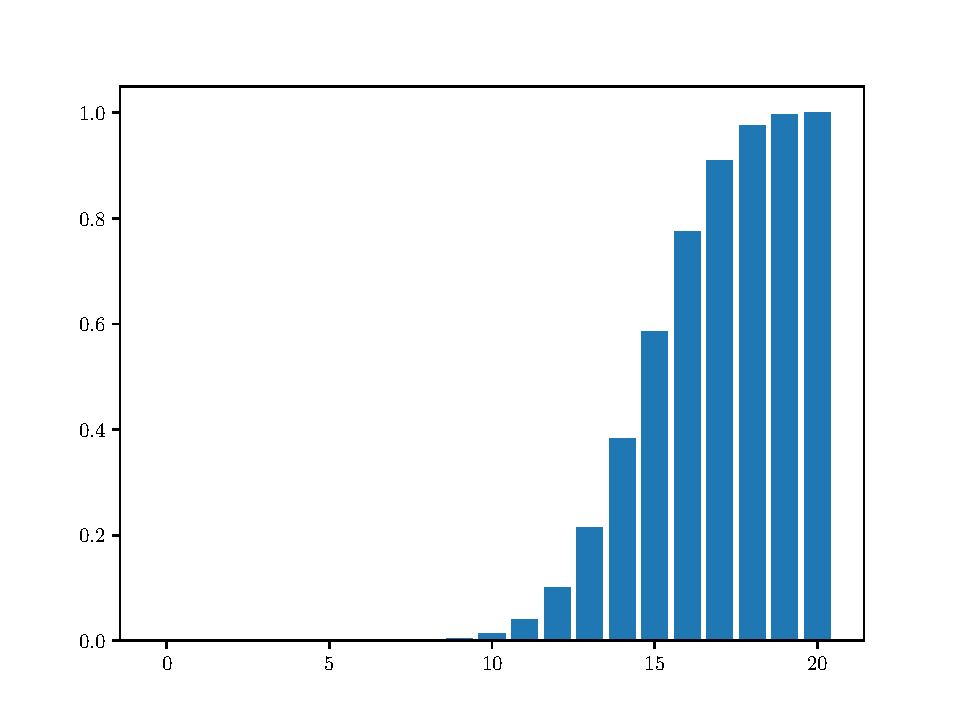
\includegraphics[width=\textwidth]{discrete/binomial/cdf_20_075.pdf}
		\caption{$B(20, 0.75)$}
	\end{subfigure}
	\begin{subfigure}[b]{0.45\textwidth}
		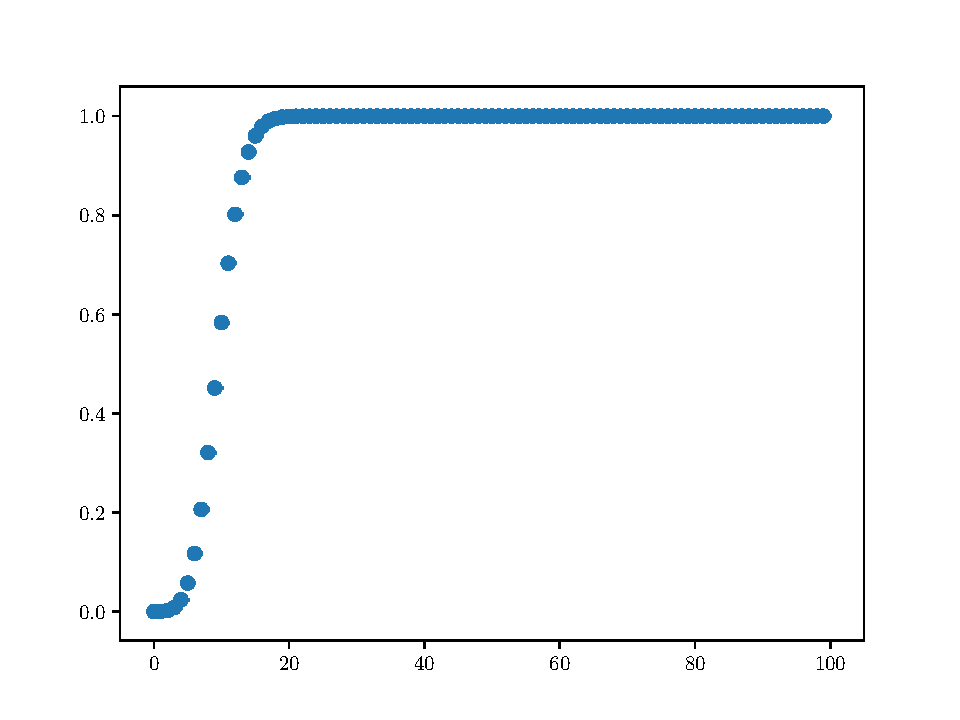
\includegraphics[width=\textwidth]{discrete/binomial/cdf_100_01.pdf}
		\caption{$B(100, 0.1)$}
	\end{subfigure}
	\begin{subfigure}[b]{0.45\textwidth}
		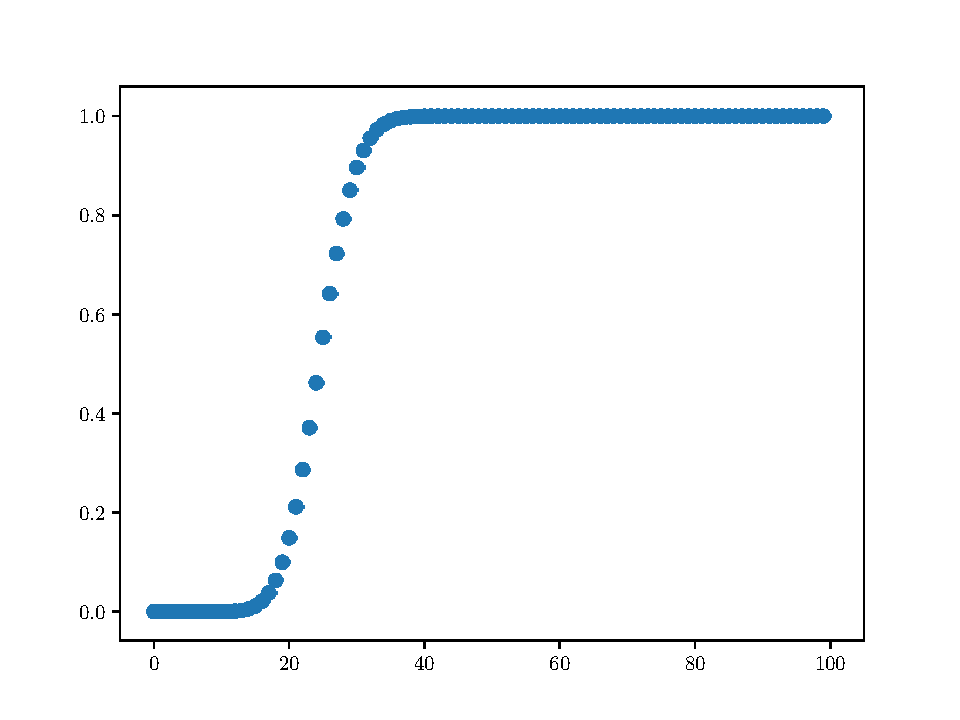
\includegraphics[width=\textwidth]{discrete/binomial/cdf_100_025.pdf}
		\caption{$B(100, 0.25)$}
	\end{subfigure}
	\caption{Binomial distribution}
\end{figure}

\begin{figure}[H]
	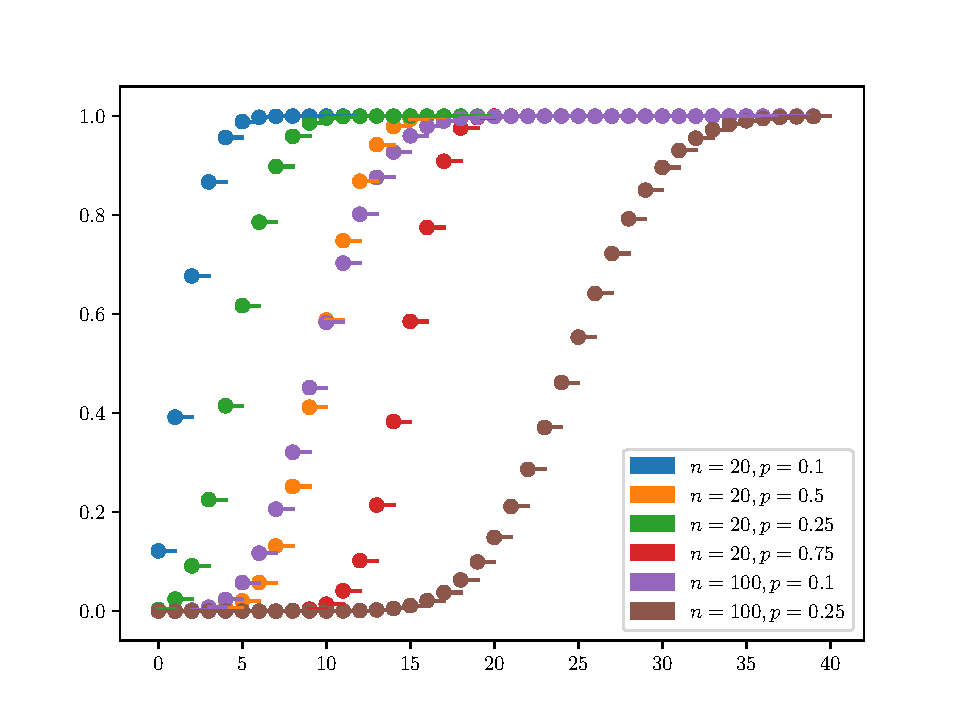
\includegraphics[width=\textwidth]{discrete/binomial/cdf_all.pdf}
	\caption{$P(X \leq k \mid n, p) = \sum_{i = 0}^{k} \binom{n}{i}p^{i}(1 - p)^{n - i}, \quad k = 0, 1, \ldots, n$}
\end{figure}

\section{Moments}

\begin{tabularx}{\textwidth}{s X}
	\hline
	Mean & $np$ \\\hline
	Variance & $np(1 - p)$\\\hline
\end{tabularx}

\section{Properties}
\begin{enumerate}
	\item Let $X_1, \ldots, X_m$ be independent random variables with $X_i \sim B(n_i, p), \ i = 1, 2, \ldots, m$. Then,
	\[
	\sum_{i = 1}^m X_i \sim B\left(\sum_{i = 1}^m n_i, p\right)
	\]
	\item Let $X_1, \ldots, X_m$ be independent Bernoulli$(p)$ random variables with success probability $p$. That is: $P(X_i = 1) = p, \ P(X_i = 0) = 1 - p, \ i = 1, \ldots, n$. Then,
	\[
	\sum_{i = 1}^m X_i \sim B\left(n, p\right)
	\]
\end{enumerate}

\section{Examples}
\begin{example}
	A fair die is rolled $n$ times.
	\begin{itemize}
		\item The probability of obtaining exactly one 6 is $n\left(\frac{1}{6}\right)\left(\frac{5}{6}\right)^{n - 1}$.
		\item The probability of obtaining no 6 is $\left(\frac{5}{6}\right)^n$.
		\item The probability of obtaining at least one 6 is $1 - \left(\frac{5}{6}\right)^n$.
		\item The number of trials needed for the probability of at least one 6 to be $\geq \frac{1}{2}$ is given by the smallest integer $n$ such that $1 - \left(\frac{5}{6}\right)^n \geq \frac{1}{2}$, so that $n \geq \frac{\log 2}{\log 1.2} \approx 3.8$.
	\end{itemize}
\end{example}


	\newpage

	\section{Poisson distribution}
	\subsection{Description}
The Poisson distribution expresses the probability of a given number of events occurring in a fixed interval of time or space if these events occur with a known constant mean rate and independently of the time since the last event. The Poisson distribution can also be used for the number of events in other specified intervals such as distance, area or volume.

For instance, an individual keeping track of the amount of mail they receive each day may notice that they receive an average number of 4 letters per day. If receiving any particular piece of mail does not affect the arrival times of future pieces of mail, i.e., if pieces of mail from a wide range of sources arrive independently of one another, then a reasonable assumption is that the number of pieces of mail received in a day obeys a Poisson distribution. Other examples that may follow a Poisson distribution include the number of phone calls received by a call center per hour, the number of decay events per second from a radioactive source, the number of visits to a website and the number of typographical errors per page in a book.

The Poisson distribution is an appropriate model if the following assumptions are true:

\begin{itemize}
	\item k is the number of times an event occurs in an interval and k can take values 0, 1, 2, ....
	\item The occurrence of one event does not affect the probability that a second event will occur. That is, events occur independently.
	\item The average rate at which events occur is constant.
	\item Two events cannot occur at exactly the same instant; instead, at each very small sub-interval exactly one event either occurs or does not occur.
\end{itemize}


\subsubsection{Probability mass function}
Let $X$ denote the number of events in a unit interval of time or in a unit distance.Then, $X$ is called the Poisson random variable with mean number of events $\lambda$ in a unit interval of time. The probability mass function of a Poisson distribution with mean $\lambda$ is given by
\[
 	f(k \mid \lambda) = P(X = k \mid \lambda) = \frac{e^{-\lambda} \lambda^k}{k!}, \ k = 0, 1, 2, \ldots
\]

\subsubsection{Cumulative distribution function}
\[
	F(k \mid \lambda) = P(X = k \leq \lambda) = \sum_{i = 0}^{k} \frac{e^{-\lambda} \lambda^i}{i!}, \ k = 0, 1, 2, \ldots
\]

The Poisson distribution can also be developed as a limiting distribution of the binomial, in which $n \rightarrow \infty$ and $p \rightarrow 0$ so that $np$ remains a constant. In other words, for large $n$ and small $p$, the binomial distribution can be approximated by the Poisson distribution with mean $\lambda = np$.

If the sample was drawn without replacement from a small finite population, the hypergeometric distribution should be used instead of the binomial.

\subsection{Moments}

\begin{tabular}{p{0.5\textwidth} p{0.5\textwidth}}
	\hline
	Mean & $\lambda$ \\\hline
	Variance & $\lambda$\\\hline
\end{tabular}

\subsection{Plots}
Poisson distribution is right-skewed, and the degree of skewness decreases as $\lambda$ increases.

\begin{figure}[H]
	\centering
	\begin{subfigure}[b]{0.45\textwidth}
		\includegraphics[width=\textwidth]{poisson/P2.png}
		\caption{$\lambda = 2$}
		\label{fig:P2}
	\end{subfigure}
	\begin{subfigure}[b]{0.45\textwidth}
	\includegraphics[width=\textwidth]{poisson/P3.png}
	\caption{$\lambda = 3$}
	\label{fig:P3}
	\end{subfigure}
	\begin{subfigure}[b]{0.45\textwidth}
		\includegraphics[width=\textwidth]{poisson/P5.png}
		\caption{$\lambda = 5$}
		\label{fig:P5}
	\end{subfigure}
	\begin{subfigure}[b]{0.45\textwidth}
		\includegraphics[width=\textwidth]{poisson/P10.png}
		\caption{$\lambda = 10$}
		\label{fig:P10}
	\end{subfigure}
	\begin{subfigure}[b]{0.45\textwidth}
		\includegraphics[width=\textwidth]{poisson/P20.png}
		\caption{$\lambda = 20$}
		\label{fig:P20}
	\end{subfigure}
	\begin{subfigure}[b]{0.45\textwidth}
		\includegraphics[width=\textwidth]{poisson/P30.png}
		\caption{$\lambda = 30$}
		\label{fig:P30}
	\end{subfigure}
	\caption{Poisson distribution}\label{fig:poisson}
\end{figure}

	\newpage

	\part{Continuous distributions}
	
	%%%%%%%%%%%%%%%%%%%%%%%%%%%%%%%%%%%%%%%%%%%%%%%%%%%%%%%%%%%%%%%%%%%%%%%%%%%%%%%%%%%%%%%%%
	
\end{document}